 \thispagestyle{gocconone}
\pagestyle{gocco}
\everymath{\color{gocco}}
\graphicspath{{../gocco/pic/}}
\blfootnote{$^1${\color[named]{gocco}Tp. Hồ Chí Minh.}}
\begingroup
\AddToShipoutPicture*{\put(0,616){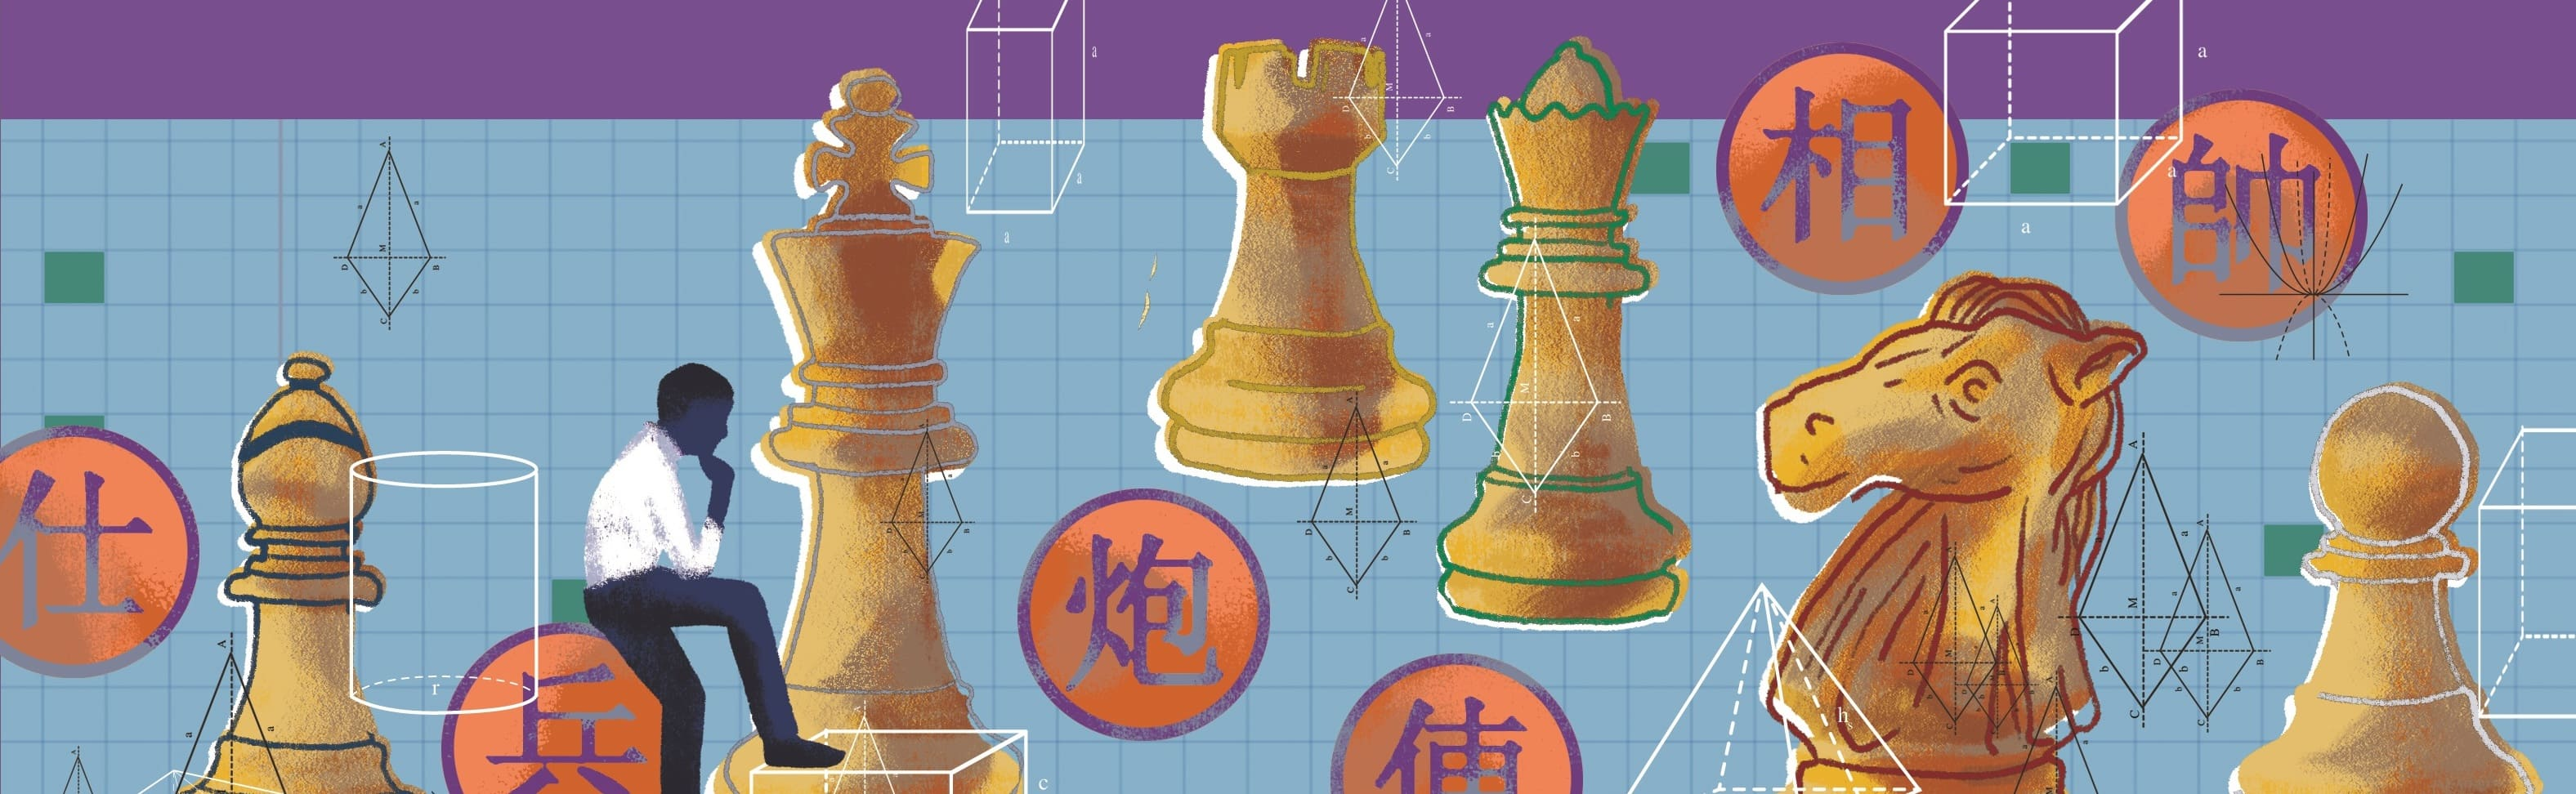
\includegraphics[width=19.3cm]{../bannergocco}}}
\AddToShipoutPicture*{\put(121,530){
\includegraphics[scale=0.95]{../tieude2.pdf}}} 
\centering
\endgroup

\vspace*{175pt}
\begin{multicols}{2}
	Tàn cuộc Pháo Chốt -- mặc dù vẫn được coi là một trong những loại hình tàn cuộc căn bản, thế nhưng việc điều quân như thế nào để đạt kết quả tốt nhất vẫn luôn  là bài toán khó đối với nhiều kỳ thủ, đặc biệt là đối với những người chơi còn thiếu kinh nghiệm thực chiến. Như những bài viết ở các số trước, chúng ta đã biết rằng, $2$ loại binh chủng Pháo và Chốt đều có những điểm yếu cố hữu của riêng mình: Chốt di chuyển từng bước một, không có khả năng đi lùi khi tiến sâu vào đất địch; Pháo có thể trở nên vô hại nếu như không có quân làm ``ngòi". 
	\vskip 0.05cm
	Để sử dụng và phối hợp $2$ quân nói trên trong tàn cuộc để đi đến thắng lợi sau cùng, ngoài việc hiểu rõ về đặc điểm và tính năng của chúng người chơi cần lưu ý một số vấn đề quan trọng để giành lấy kết quả có lợi cho ván đấu như sau:
	\vskip 0.05cm
	\textit{$1.$	Khi đổi quân, cần cân nhắc kỹ giữ Pháo hay giữ Chốt}
	\vskip 0.05cm
	Nếu như cuộc cờ đang trong giai đoạn giằng co, việc giữ Pháo là sự ưu tiên lựa chọn của đa số kỳ thủ, thế nhưng đến giai đoạn tàn cuộc mọi thứ có thể thay đổi hoàn toàn. Quân Chốt một khi áp sát cửu cung có thể được đánh giá cao hơn quân Pháo không có ``ngòi", hãy suy nghĩ thấu đáo trước khi tiến hành trao đổi.
	\vskip 0.1cm
	\textit{$2.$	Tận dụng tối đa vai trò của Sỹ, Tượng}
	\vskip 0.1cm
	Bước vào Tàn cuộc, số lượng quân chiến đôi bên không còn nhiều, việc giữ Sỹ, Tượng và tận dụng chúng để hỗ trợ cho Pháo là điều vô cùng cần thiết. Trong nhiều tình huống, chúng góp phần làm thay đổi kết quả sau cùng của ván cờ.
	\vskip 0.1cm
	\textit{$3.$	Chú ý dùng Tướng chiếm mặt đúng thời điểm}
	\vskip 0.1cm
	Tướng là đối tượng luôn được ưu tiên bảo vệ trong mọi tình huống, nhưng trong các loại hình tàn cuộc nói chung và tàn Pháo Chốt nói riêng, kỳ thủ cần phải  biết tận dụng mặt Tướng để chiếm lộ, hạn chế khả năng hoạt động cũng như truy sát Tướng đối phương.
	\vskip 0.1cm
	\textit{$4.$	Nắm bắt tính chẵn--lẻ của nước đi. đẩy đối phương vào thế khó.}
	\vskip 0.1cm
	Nghe qua thì có vẻ không mấy liên quan vì khái niệm chẵn lẻ chỉ thường xuất hiện trong Toán học. Nhưng đôi khi trong các ván đấu cờ Tướng, đặc biệt trong cờ tàn Pháo Chốt, các kỳ thủ cần lợi dụng đặc điểm này để thực hiện nước nhấp một cách hợp lý, biến lượt đi của mình thành lượt đi đối phương, ép buộc đối phương phải đi quân để tự rơi vào tình huống bất lợi, từ đó giành lấy thắng lợi sau cùng.
	\vskip 0.1cm
	Để hiểu hơn về những điểm nêu trên, trong bài viết kỳ này, tác giả xin gửi đến bạn đọc Pi một số hình tàn cuộc Pháo Chốt đặc sắc, từ đó có thể áp dụng vào thực chiến:
	\begin{figure}[H]
		\vspace*{-5pt}
		\centering
		\captionsetup{labelformat= empty, justification=centering}
		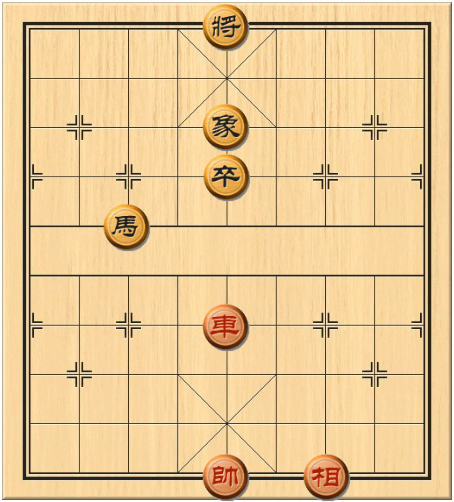
\includegraphics[width= 0.4\textwidth]{1}
		\caption{\small\textit{\color{gocco}Hình $1$.}}
		\vspace*{-10pt}
	\end{figure}
	$1.$	Hình $1$, Đỏ còn Pháo Chốt,Đen chỉ còn đơn Tượng, Đỏ khéo léo giành chiến thắng như sau: 
	\vskip 0.1cm
	$\pmb{1)}$	P$2-8$ T$3.1$\quad $\pmb{2)}$ P$8.2(*)$ T$1/3$\quad $\pmb{3)}$ C$5.1$ T$3.1$\quad $\pmb{4)}$ Tg$4-5$ T$1/3$\quad $\pmb{5)}$ P$8.2$ Tg$4/1$\quad $\pmb{6)}$ C$5-6(**)$ T$3.5$\quad $\pmb{7)}$ C$6-5$ $(1-0)$
	\vskip 0.1cm
	\textit{$(*)$: Với sự cơ động của Pháo, Đỏ lập tức đem qua cánh còn lại nhằm cản trở nước đi của Tượng đối phương.
	\vskip 0.1cm
	$(**)$: Tiếp theo đó, Đỏ dùng Tướng chiếm trung lộ để bình chốt, thu hẹp không gian hoạt động của Tướng và Tượng Đen. Đen thua do không còn quân đi.}
	\vskip 0.1cm
	$2.$	Hình $2$, Bên Đỏ còn Pháo Chốt đang nắm lợi thế lớn, tuy nhiên, với Chốt đã xuống sâu thì việc giành chiến thắng xem ra cũng không hề đơn giản. Đỏ đã áp dụng các quy tắc và ra đòn như sau:
	\vskip 0.1cm
	$\pmb{1)}$	P$5-2$ St$/5$\quad $\pmb{2)}$ P$2.8(*)$ S$5.4$\quad $\pmb{3)}$ C$3-4$ St$/5$\quad $\pmb{4)}$ P$2-5$ S$5.6$\quad $\pmb{5)}$ Tg$4/1$ Tg$5-4$\quad $\pmb{6)}$ Tg$4-5(**)$ S$6/5$\quad $\pmb{7)}$ P$5-2$ S$5.6$\quad $\pmb{8)}$ P$2/1$ S$6/5$\quad $\pmb{9)}$ P$2-5(***)$ S$4.5$\quad $\pmb{10)}$ C$4-5$ $(1-0)$
	\begin{figure}[H]
		\vspace*{5pt}
		\centering
		\captionsetup{labelformat= empty, justification=centering}
		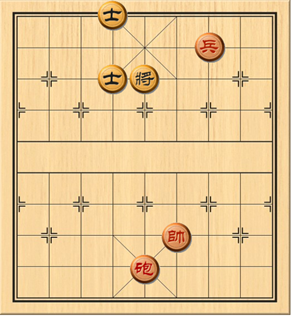
\includegraphics[width= 0.4\textwidth]{2}
		\caption{\small\textit{\color{gocco}Hình $2$.}}
		\vspace*{-10pt}
	\end{figure}
	\textit{$(*)$: Trong bối cảnh không còn Sỹ Tượng để làm ngòi, Đỏ bình Pháo rồi tấn Pháo xuống đáy, thể hiện ý đồ rõ ràng nhằm di chuyển vào giữa và chiếm lấy trung lộ. 
	\vskip 0.1cm
	$(**)$: Sau khi bình Chốt áp sát và bình Pháo vào đường $5$, Đỏ có nước thoái Tướng chờ đợi đầy tinh tế. Đen không còn nước hay để đi đành bình Tướng, nhường lại cho Đỏ trục lộ quan trọng.
	\vskip 0.1cm
	$(***)$: Mục tiêu ban đầu đã hoàn thành, Đỏ nhanh chóng điều Pháo trở về hàng áp đáy, dùng Pháo đổi $2$ Sỹ để giành lấy thắng lợi. Nếu lúc này sai lầm dùng Chốt ăn Sỹ, sẽ trở thành cờ hòa ngay lập tức.}
	\begin{figure}[H]
		\vspace*{-5pt}
		\centering
		\captionsetup{labelformat= empty, justification=centering}
		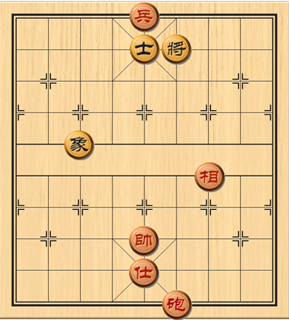
\includegraphics[width= 0.4\textwidth]{3}
		\caption{\small\textit{\color{gocco}Hình $3$.}}
		\vspace*{-5pt}
	\end{figure}
	$3.$ Hình $3$, mặc dù Đỏ đang có lợi thế nhưng để có thể giành chiến thắng  hình cờ này đòi hỏi kỳ thủ cần phải nắm vững các kỹ thuật khóa quân và lấy mặt Tướng trong Tàn cuộc Pháo Chốt. Đỏ đi:
	\vskip 0.1cm
	$\pmb{1)}$	S$5.4$ S$5.6$\quad $\pmb{2)}$ Tg$5/1(*)$ T$3/5$\quad $\pmb{3)}$ P$4-3$ T$5.3$\quad $\pmb{4)}$ P$3-5$ T$3/1$\quad $\pmb{5)}$ T$3/5$ T$1.3$\quad $\pmb{6)}$ T$5.7$ T$3/1$\quad $\pmb{7)}$ P$5-7(**)$ S$6/5$\quad $\pmb{8)}$ Tg$5/1$ S$5.6$\quad $\pmb{9)}$ P$7.3$ S$6/5$\quad $\pmb{10)}$ P$7/2$ S$5.6$\quad $\pmb{11)}$ C$5-6$ S$6/5$\quad $\pmb{12)}$ P$7-4$ S$5.6$\quad $\pmb{13)}$ Tg$5-4$ T$1.3$\quad $\pmb{14)}$ P$4-7$ T$3/1$\quad $\pmb{15)}$ S$4/5$ Tg$6-5$\quad $\pmb{16)}$ S$5.6$ Tg$5.1$\quad $\pmb{17)}$ Tg$4.1$ S$6/5$\quad $\pmb{18)}$ P$7-6$ S$5.6$\quad $\pmb{19)}$ P$6/1$ S$6/5$\quad $\pmb{20)}$ T$7/5$ S$5.6$\quad $\pmb{21)}$ P$6-4(****)$ S$6/5$\quad $\pmb{22)}$ P$4-5$ (Đỏ mất Sỹ, $1-0$)
	\vskip 0.1cm
	\textit{$(*)$: Sau khi dùng Sỹ làm ngòi uy hiếp Tướng Đen, Đỏ lùi Tướng nhằm nhường đường cho Tượng đảo qua cánh còn lại.
	\vskip 0.1cm
	$(**)$: Những nước điều Pháo rất có ý đồ của Đỏ, khiến cho Tượng Đen phải dạt sang lộ $1$. Nhân cơ hội đó, Đỏ đã thực hiện việc treo Tượng lên lộ $7$ và bình Pháo trói chặt Tượng đối phương.
	\vskip 0.1cm
	$(***)$: Giai đoạn vừa rồi Đỏ đã thực hiện một loạt các nước đi điều quân nhằm mục đích sắp xếp đội hình trước khi ra đòn, Đen không thể làm gì hơn ngoài việc đi Sỹ. Đặc biệt, nước số $9-10$, Đỏ đã áp dụng số nước đi chẵn lẻ nhằm lấy nhịp về sau có thể bình ra bắt Tượng (nước số $14$) và mở Sỹ chiếm mặt (nước số $15$).
	\vskip 0.1cm
	$(****)$: Những nước tiếp theo Đỏ điều chuyển Tướng, Sĩ, Tượng một cách khéo léo làm ngòi cho Pháo rồi bắt chết Sĩ, cuối cùng Đen đành chấp nhận thua cuộc.}
	\vskip 0.1cm
	\textit{Chú thích}: C: Chốt, P: Pháo, Tg: Tướng, S: Sĩ, T: Tượng, t: trước, s: sau.
	\vskip 0.1cm
	\textbf{\color{gocco}Câu đố kỳ này:} Đỏ đi trước và sẽ khéo léo kết hợp Pháo Chốt như thế nào để giành lấy thắng lợi trong những hình tàn cuộc sau?
	\begin{figure}[H]
		\vspace*{5pt}
		\centering
		\captionsetup{labelformat= empty, justification=centering}
		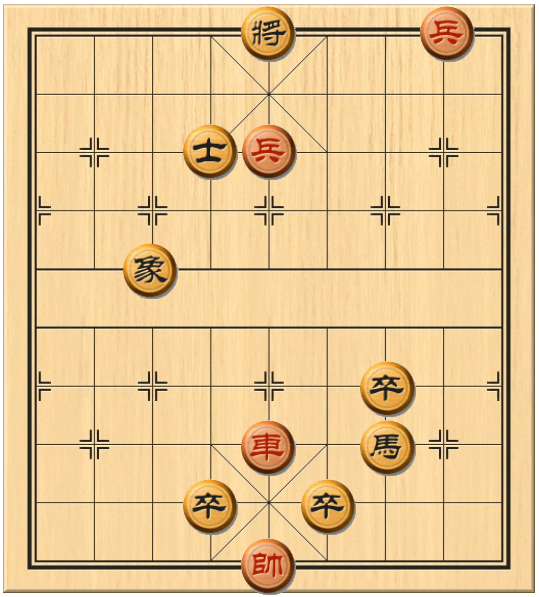
\includegraphics[width= 0.4\textwidth]{4}
		\caption{\small\textit{\color{gocco}Hình $4$.}}
		\vspace*{-10pt}
	\end{figure}
	\textit{Đáp án tham khảo:} $\pmb{1)}$ P$8/2$ T$5/7$\quad  $\pmb{2)}$ Tg$5-6$ T$7.9$\quad $\pmb{3)}$ T$3.5$ T$9.7$\quad $\pmb{4)}$ P$8-4$ T$3/5$\quad $\pmb{5)}$ C$5-4$ Tg$5.1$\quad $\pmb{6)}$ C$4.1$ T$5/3$\quad $\pmb{7)}$ C$4.1$ T$3.1$\quad $\pmb{8)}$ P$4-5$ T$7/5$\quad $\pmb{9)}$ P$5.7$ (Đen mất Tượng, Đỏ tiếp tục đưa Pháo về đáy dùng thủ đoạn tương tự bắt chết Tượng còn lại, Đỏ thắng)
	\begin{figure}[H]
		\vspace*{-5pt}
		\centering
		\captionsetup{labelformat= empty, justification=centering}
		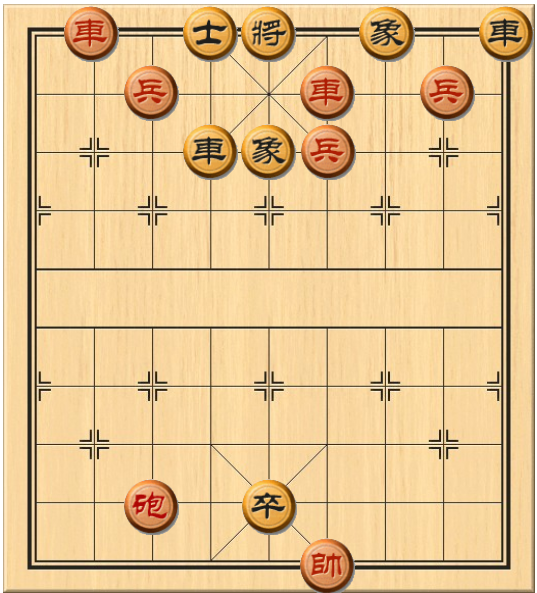
\includegraphics[width= 0.4\textwidth]{5}
		\caption{\small\textit{\color{gocco}Hình $5$.}}
		\vspace*{-10pt}
	\end{figure}
	\textit{Đáp án tham khảo:} $\pmb{1)}$ C$6.1$ T$9.7$\quad $\pmb{2)}$ P$5.3$ Ts$.9$\quad  $\pmb{3)}$ Tg$4/1$ T$9/7$\quad $\pmb{4)}$ Tg$4-5$ Ts$.9$\quad $\pmb{5)}$ Tg$5-6$ T$9/7$\quad $\pmb{6)}$ P$5-9$ S$4.5$\quad $\pmb{7)}$ Tg$6-5$ Ts$.9$\quad  $\pmb{8)}$ P$9-3$ T$7/5$\quad $\pmb{9)}$ P$3-5$ T$9/7$\quad $\pmb{10)}$ Tg$5-6$ T$7.9$\quad $\pmb{12)}$ C$6.1$ $(1-0)$
\end{multicols}




